This appendix collects the supplementary figures that the program produces but that the chapters reference rather than reproduce in full. Each one is named where it belongs in the body, and the file name printed in its caption matches the output of \code{make\_figures.py} and the figure table in \code{program/README.md}. Figures already shown in the running text are not repeated here.

\section{Search traces across the variants}\label{app:traces}

\Cref{fig:trace} in \Cref{ch:discover} follows one cooling run in detail. The runs below repeat that experiment for the other variants. Each plots every visited graph by its binding connectivity (horizontal) against its size (vertical), colouring each point by the step at which it was visited, from the hot early exploration in warm tones to the converged tail in blue. In every case the walk strays past the feasibility boundary while hot and is driven back onto the densest feasible graph as the temperature falls, exactly as in the body figure. The seeds are fixed, so each picture reproduces verbatim.

\begin{figure}[htbp]
    \centering
    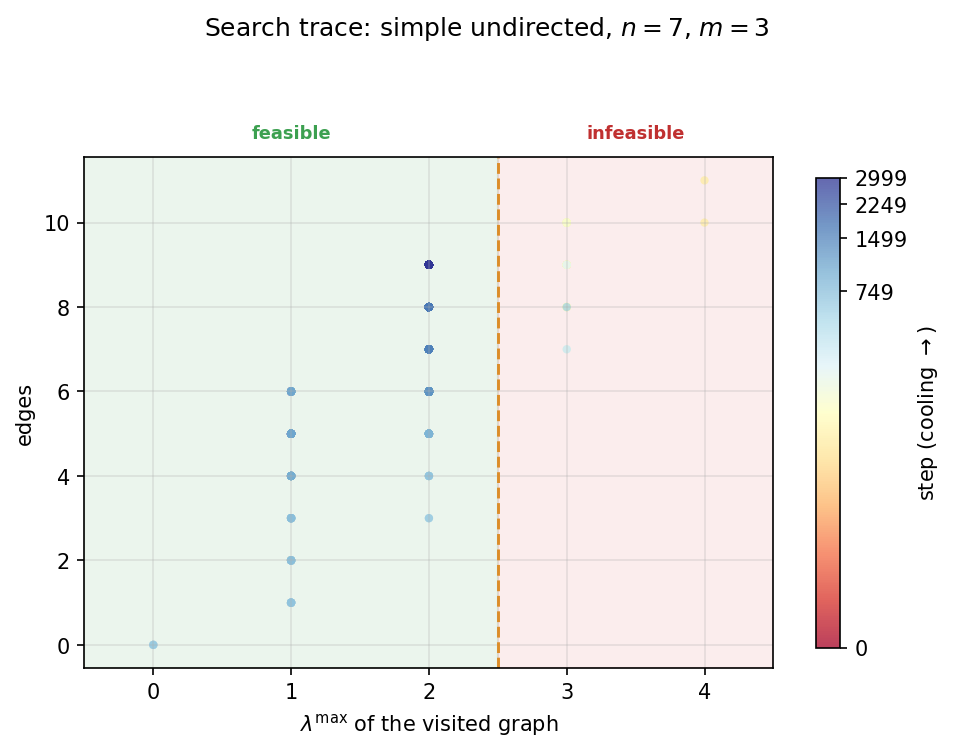
\includegraphics[width=0.74\textwidth]{figures/trace_simple_undirected_n7_m3.png}
    \caption{Search trace for the simple undirected edge problem at $n = 7$, $m = 3$. File \code{trace\_simple\_undirected\_n7\_m3.png}.}
    \label{fig:trace-simple-undirected}
\end{figure}

\begin{figure}[htbp]
    \centering
    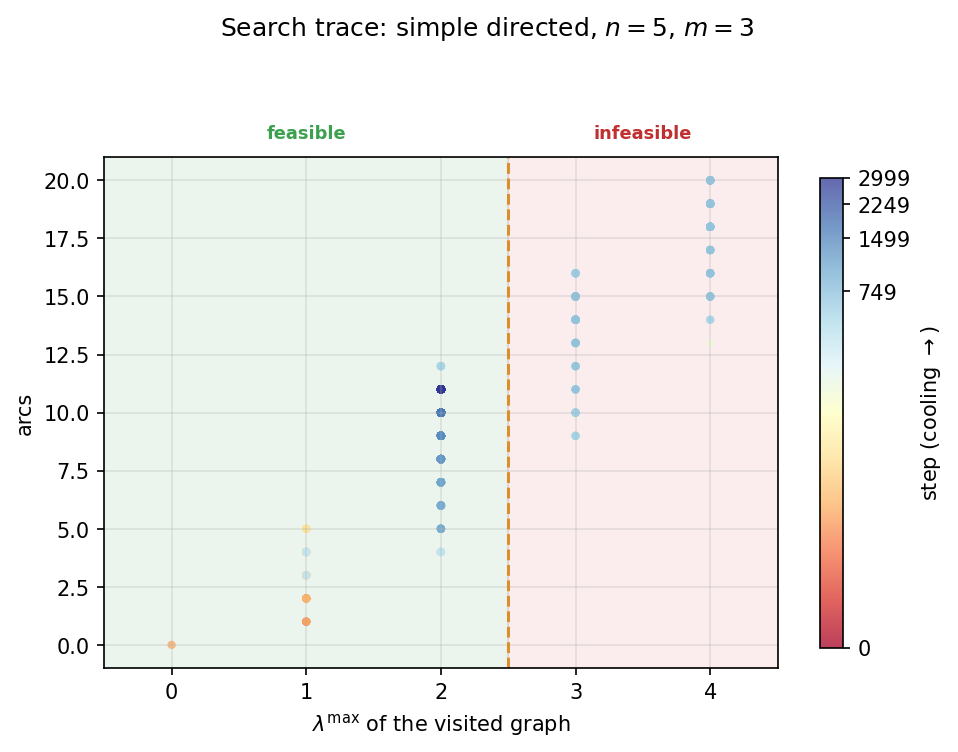
\includegraphics[width=0.74\textwidth]{figures/trace_simple_directed_n5_m3.png}
    \caption{Search trace for the simple directed arc problem at $n = 5$, $m = 3$. File \code{trace\_simple\_directed\_n5\_m3.png}.}
    \label{fig:trace-simple-directed}
\end{figure}

\begin{figure}[htbp]
    \centering
    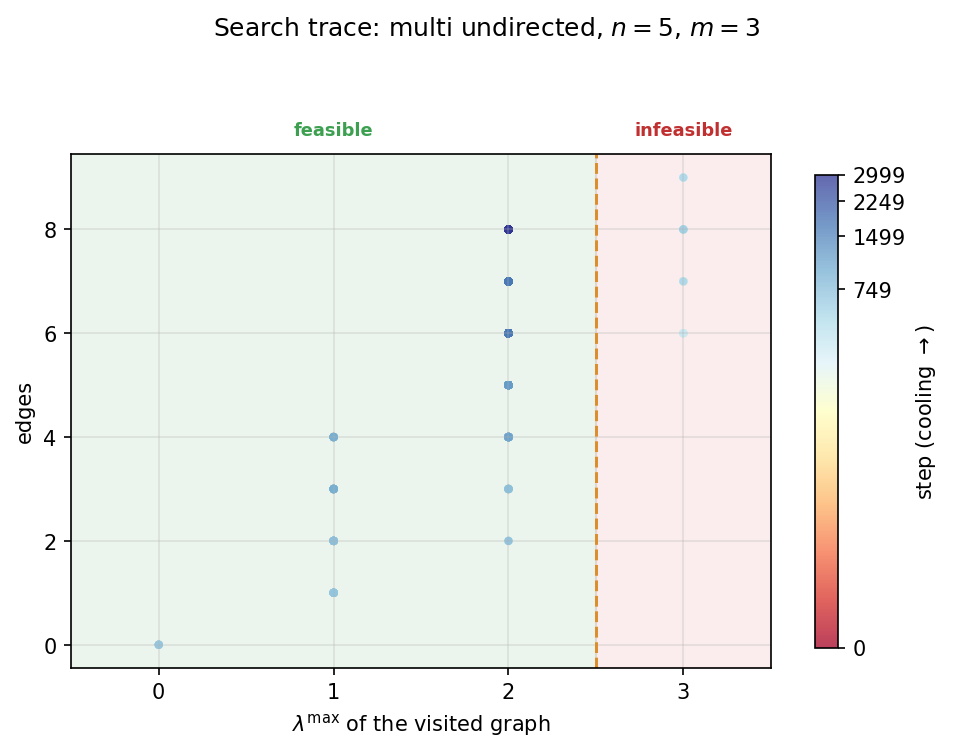
\includegraphics[width=0.74\textwidth]{figures/trace_multi_undirected_n5_m3.png}
    \caption{Search trace for the multigraph undirected edge problem at $n = 5$, $m = 3$. File \code{trace\_multi\_undirected\_n5\_m3.png}.}
    \label{fig:trace-multi-undirected}
\end{figure}

\begin{figure}[htbp]
    \centering
    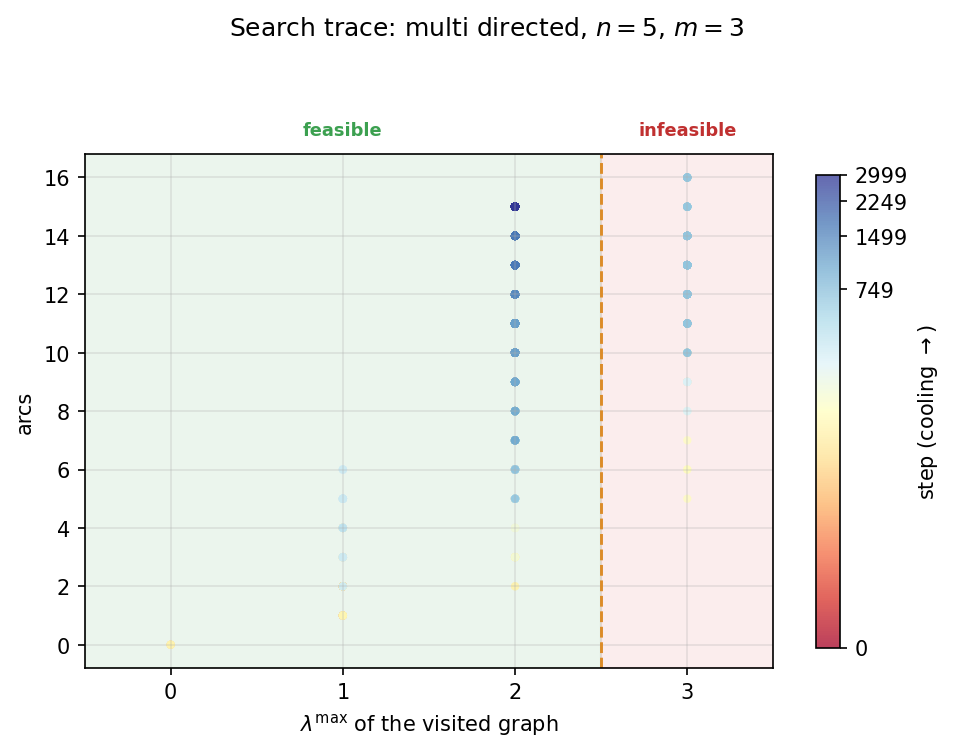
\includegraphics[width=0.74\textwidth]{figures/trace_multi_directed_n5_m3.png}
    \caption{Search trace for the multigraph directed arc problem at $n = 5$, $m = 3$. File \code{trace\_multi\_directed\_n5\_m3.png}.}
    \label{fig:trace-multi-directed}
\end{figure}

\begin{figure}[htbp]
    \centering
    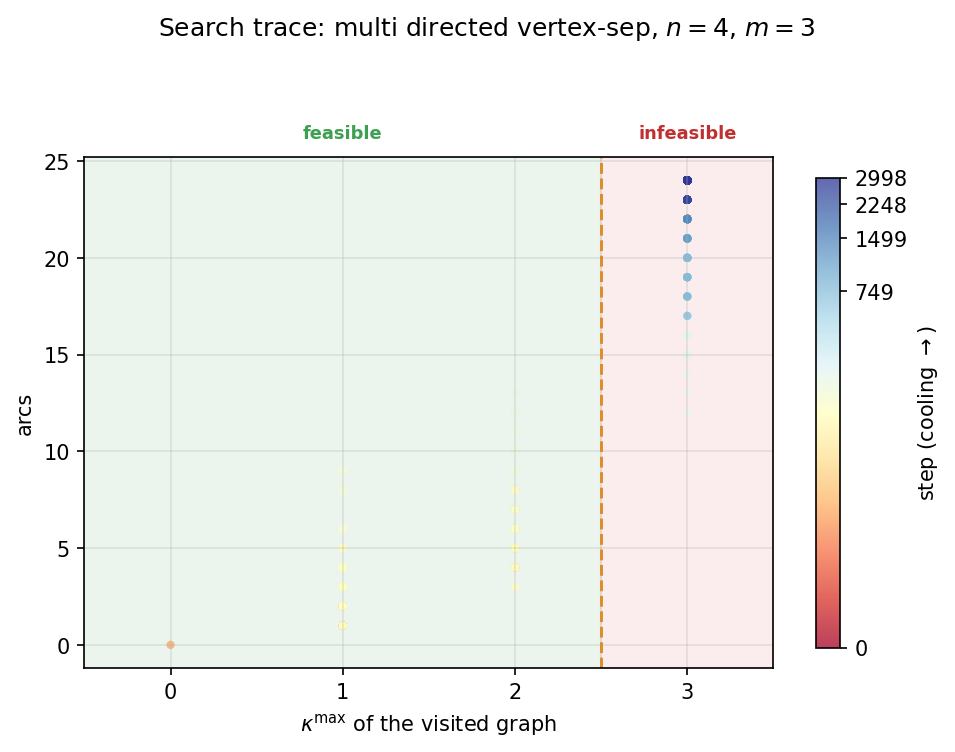
\includegraphics[width=0.74\textwidth]{figures/trace_multi_directed_n4_m3_vertex.png}
    \caption{Search trace for the multigraph directed \emph{vertex}-disjoint problem at $n = 4$, $m = 3$, where the binding quantity is $\kappa^{\max}$. File \code{trace\_multi\_directed\_n4\_m3\_vertex.png}.}
    \label{fig:trace-multi-directed-vertex}
\end{figure}

\section{The variant landscape at \texorpdfstring{$m = 6$}{m = 6} and in three dimensions}\label{app:m6}

These are the $m = 6$ companions to the $m = 3$ enumeration views of \Cref{ch:synthesis}, together with a three-dimensional view of the appearance threshold. They confirm that raising the forbidden threshold relocates the feasibility boundary without changing the qualitative picture.

\begin{figure}[htbp]
    \centering
    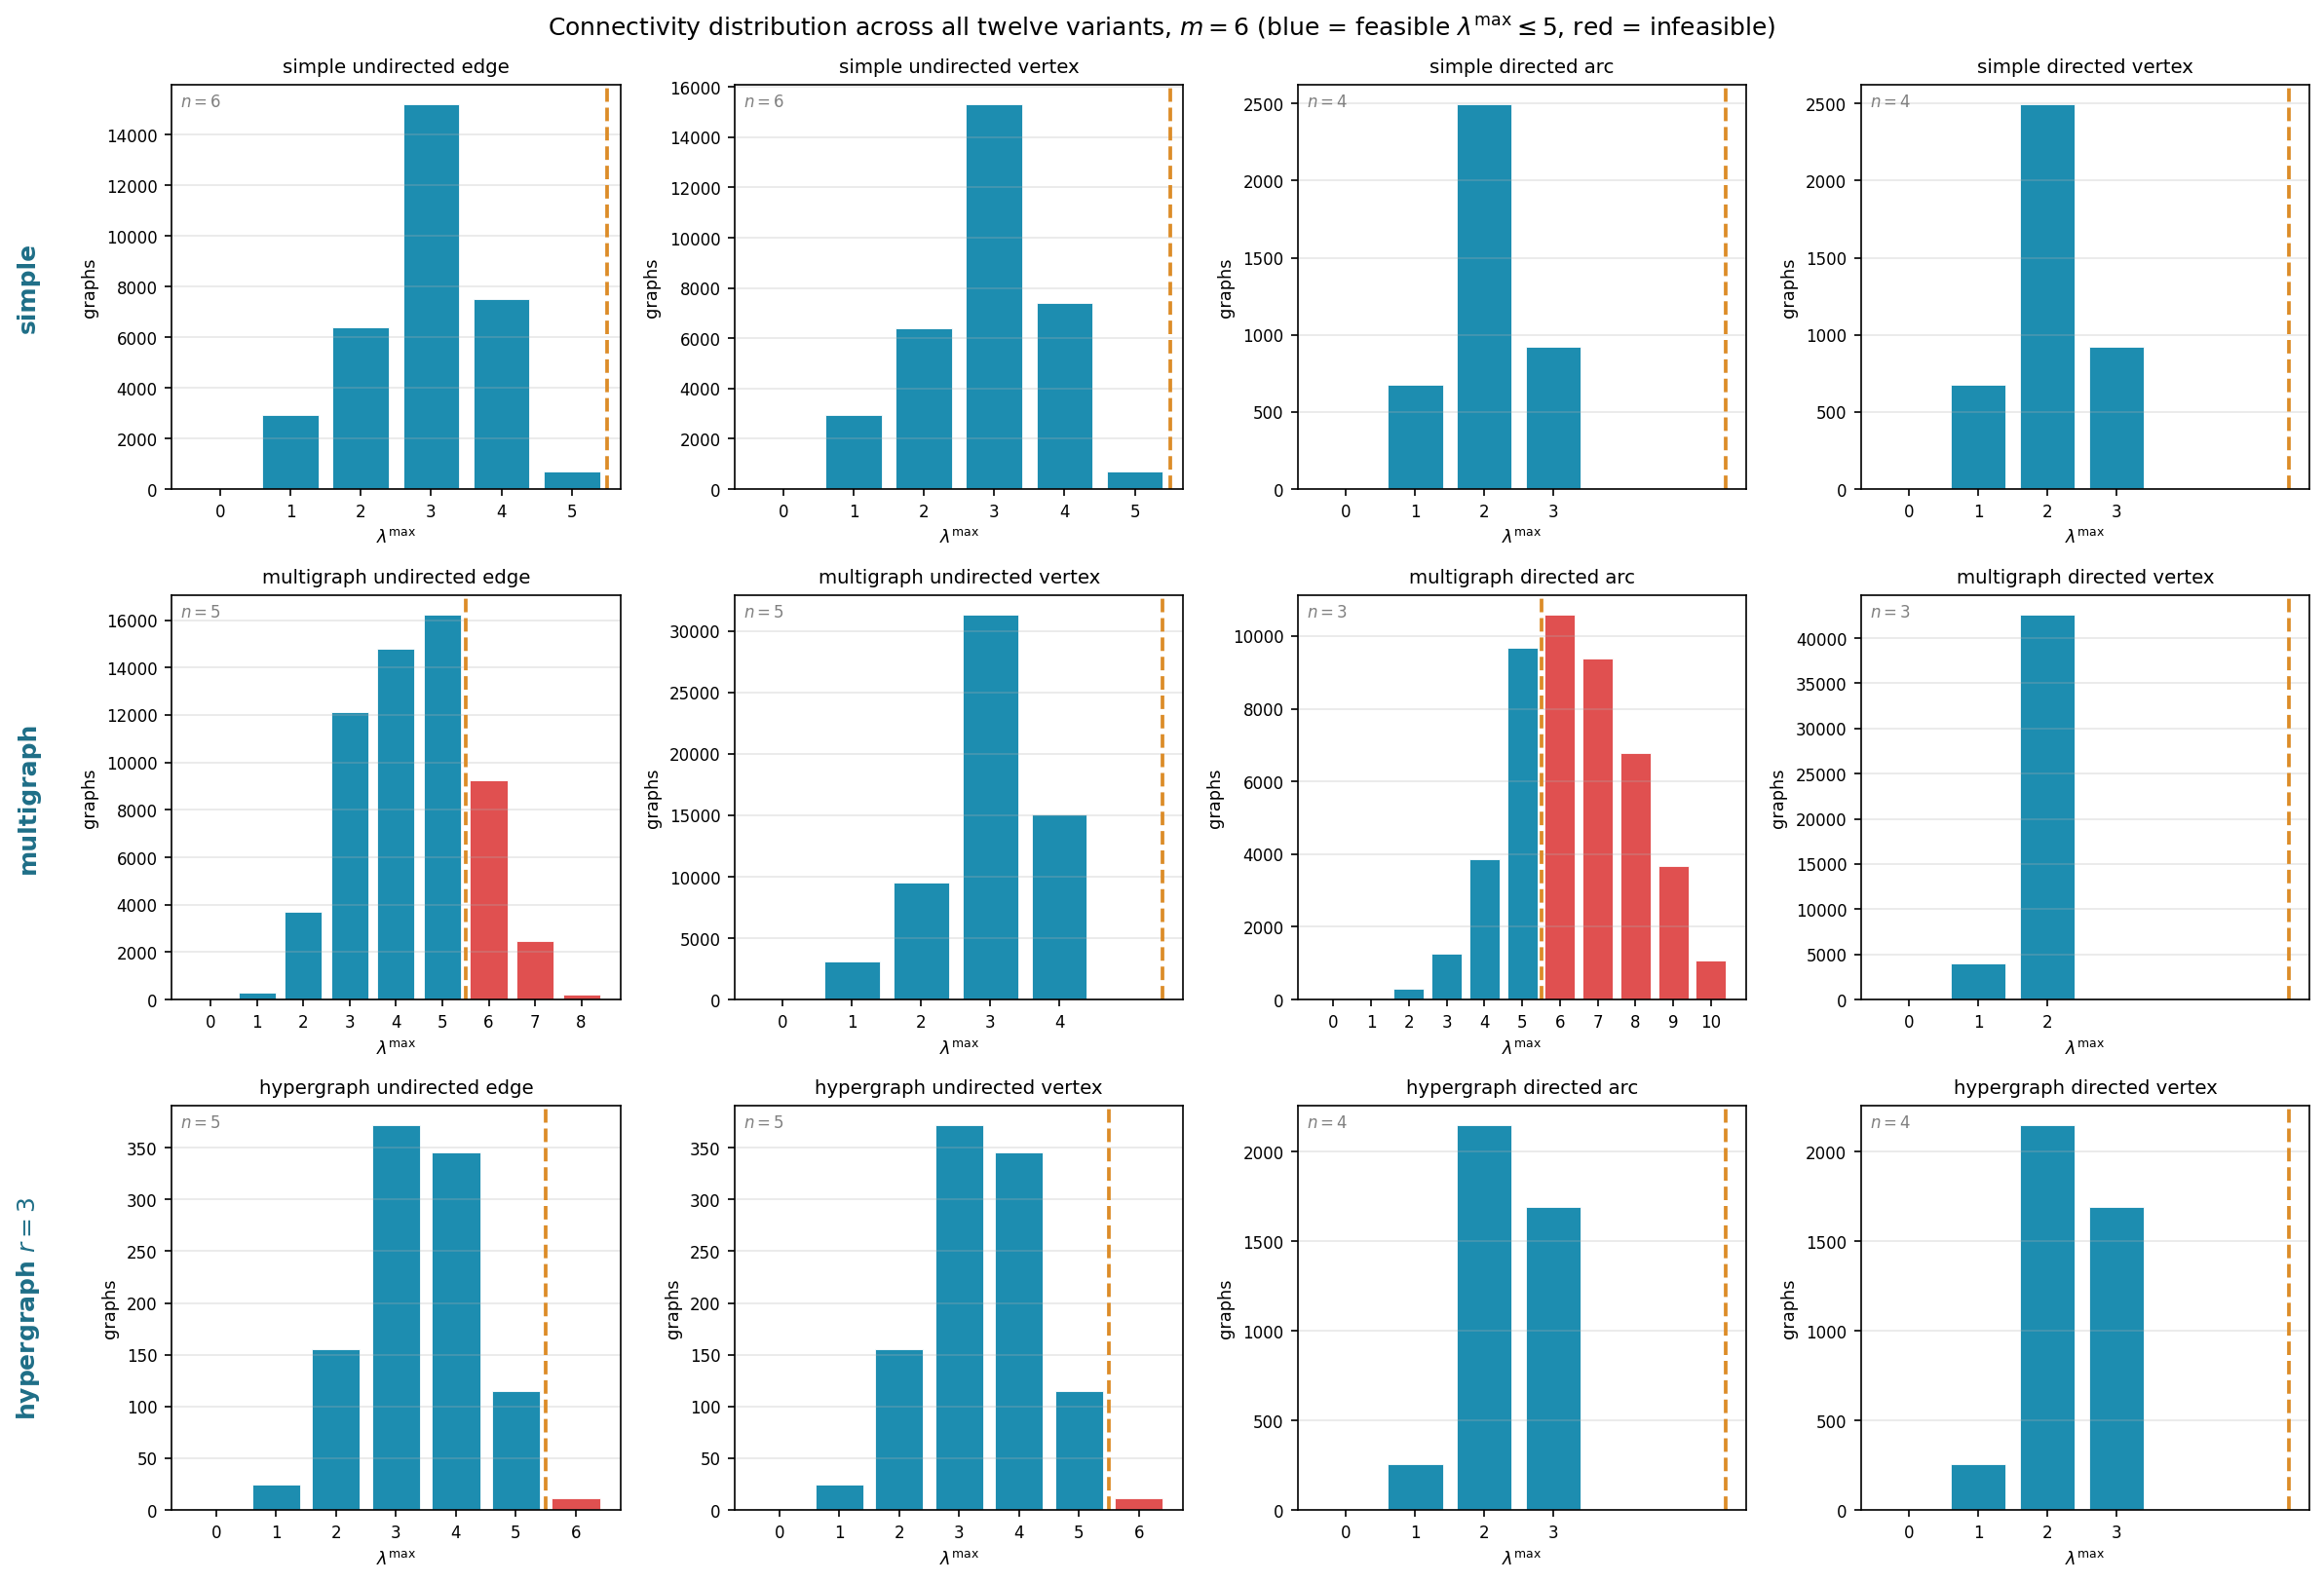
\includegraphics[width=\textwidth]{figures/conn_dist_m6.png}
    \caption{How the full small-$n$ enumeration distributes by binding connectivity $\lambda^{\max}$ across all twelve variants at $m = 6$, the companion to \Cref{fig:conn-dist-m3}. Blue bars are feasible graphs ($\lambda^{\max} \le 5$), red bars infeasible ones, and the dashed line marks the feasibility boundary. File \code{conn\_dist\_m6.png}.}
    \label{fig:conn-dist-m6}
\end{figure}

\begin{figure}[htbp]
    \centering
    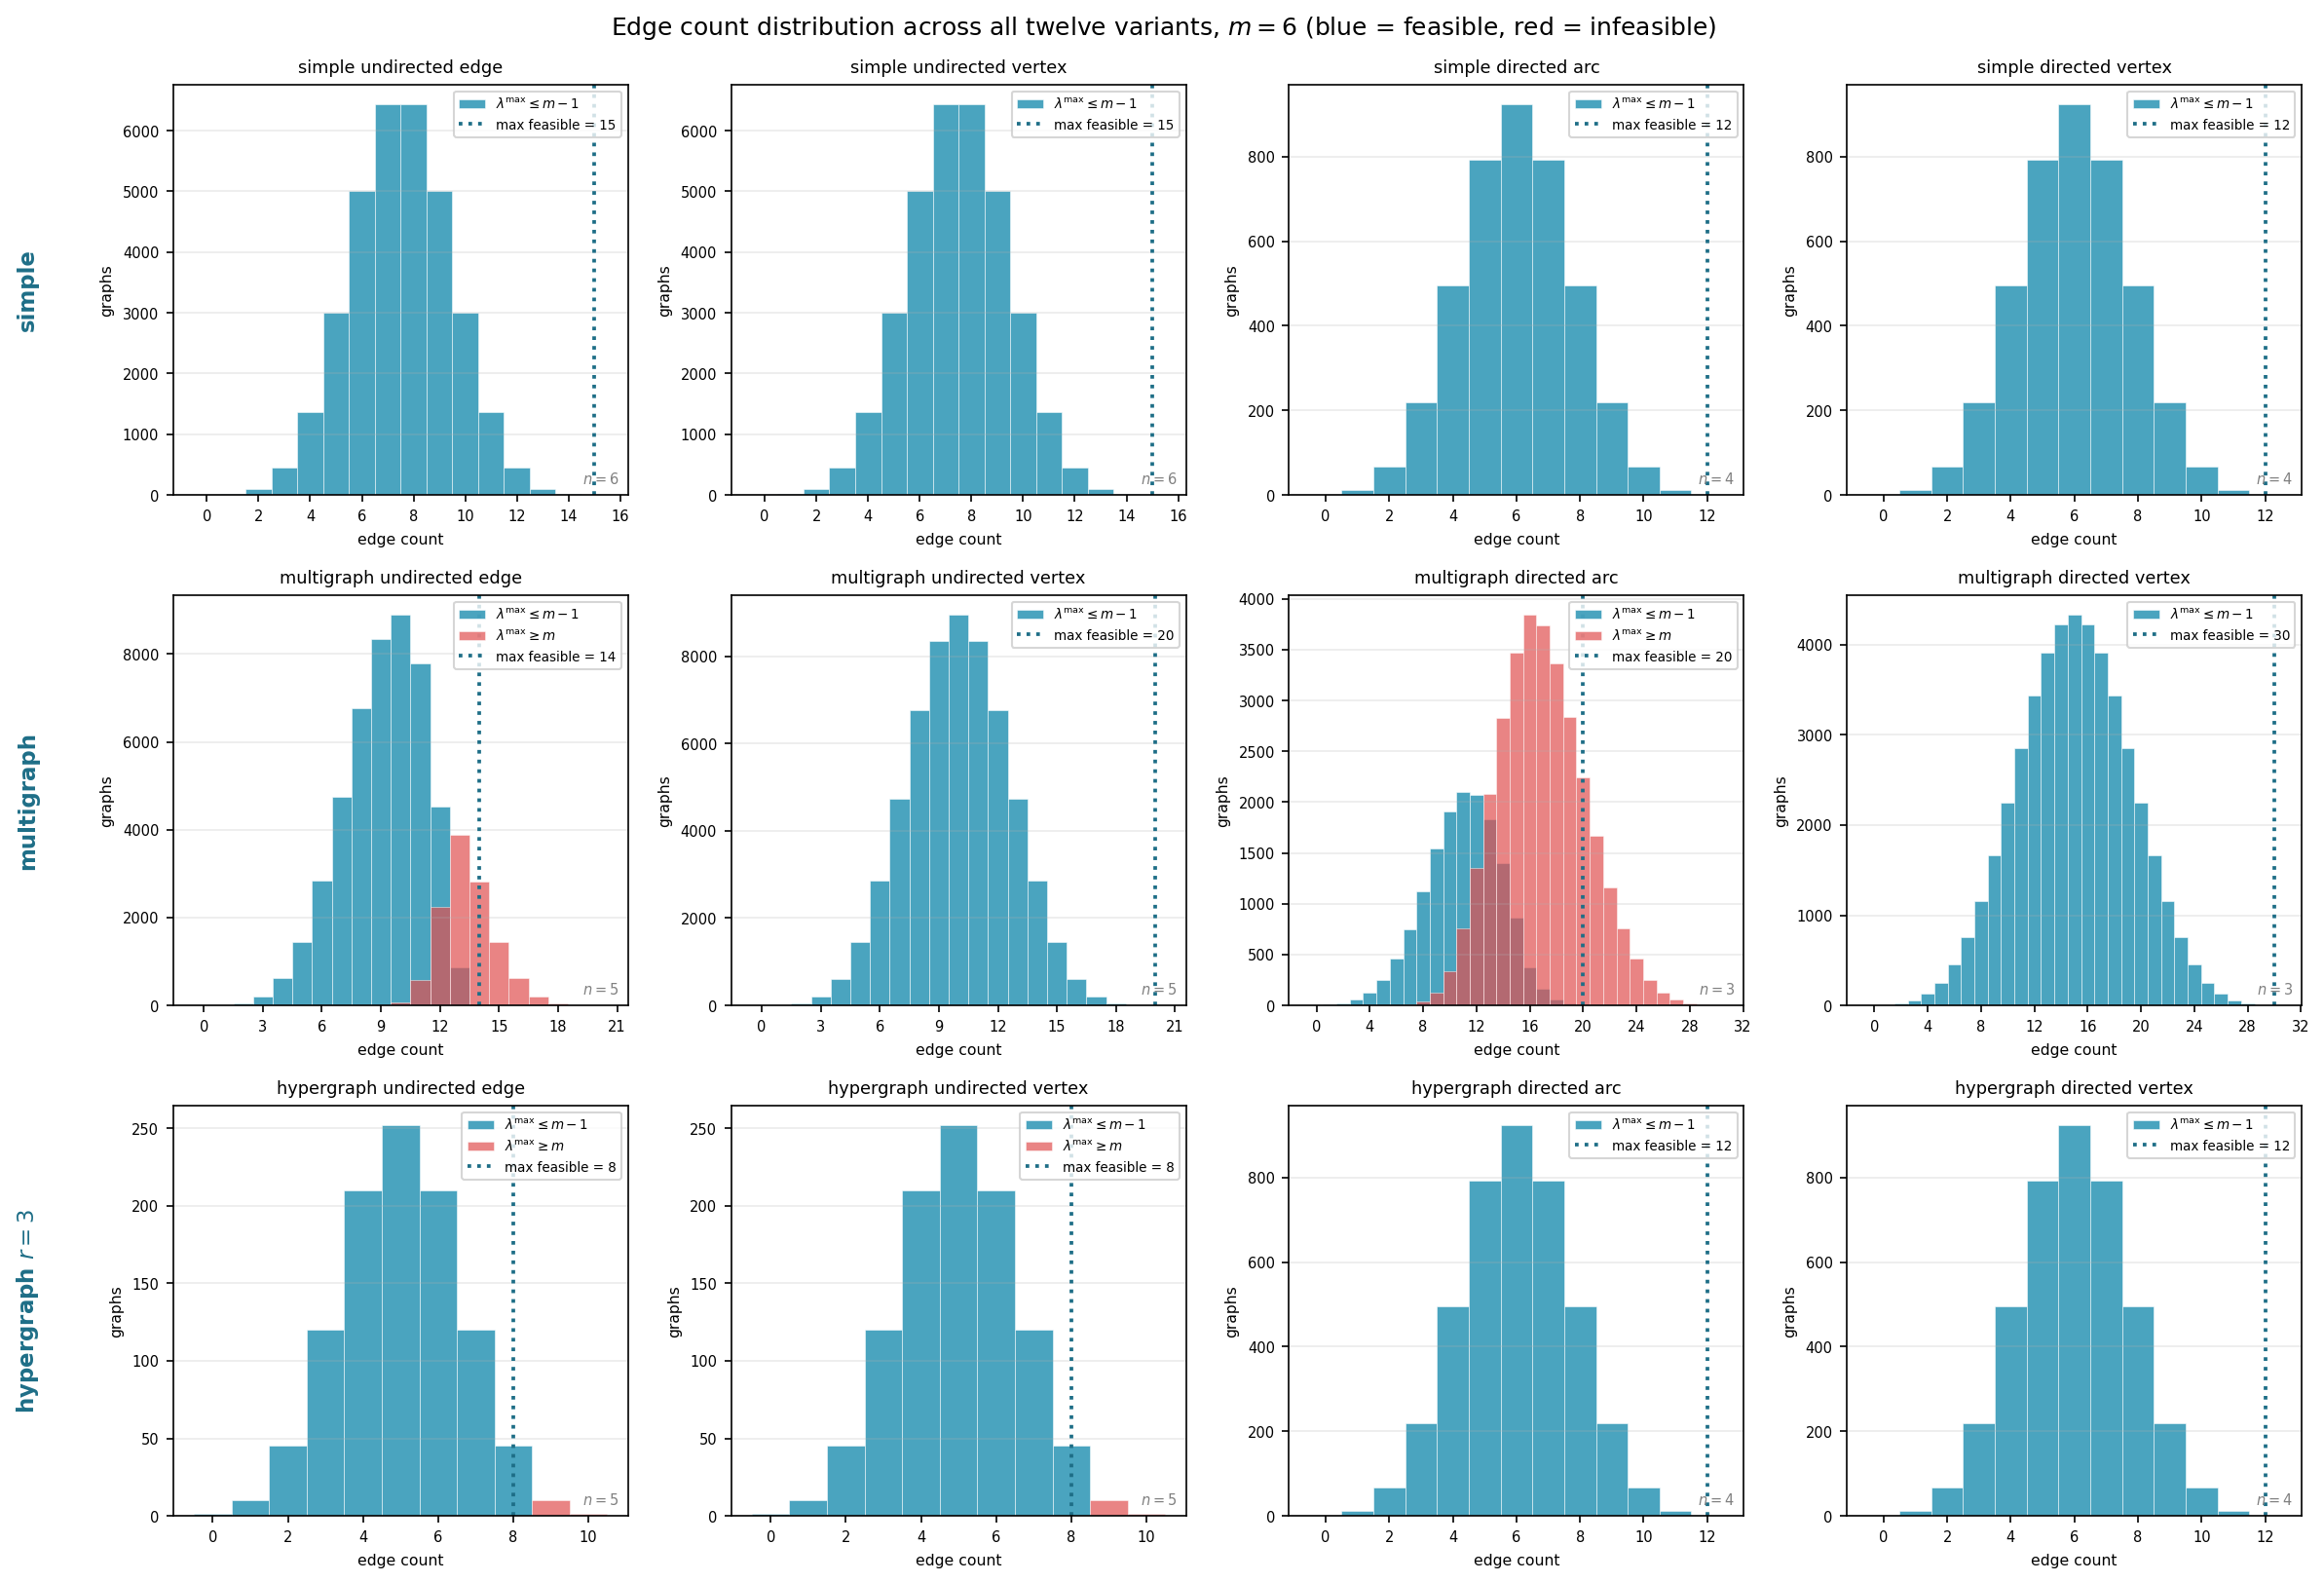
\includegraphics[width=\textwidth]{figures/edges_dist_m6.png}
    \caption{The same enumeration at $m = 6$ viewed by edge count, the companion to \Cref{fig:edge-dist-m3}. Feasible graphs are blue, infeasible ones red, and the dotted vertical line marks the extremal value at that size. File \code{edges\_dist\_m6.png}.}
    \label{fig:edge-dist-m6}
\end{figure}

\begin{figure}[htbp]
    \centering
    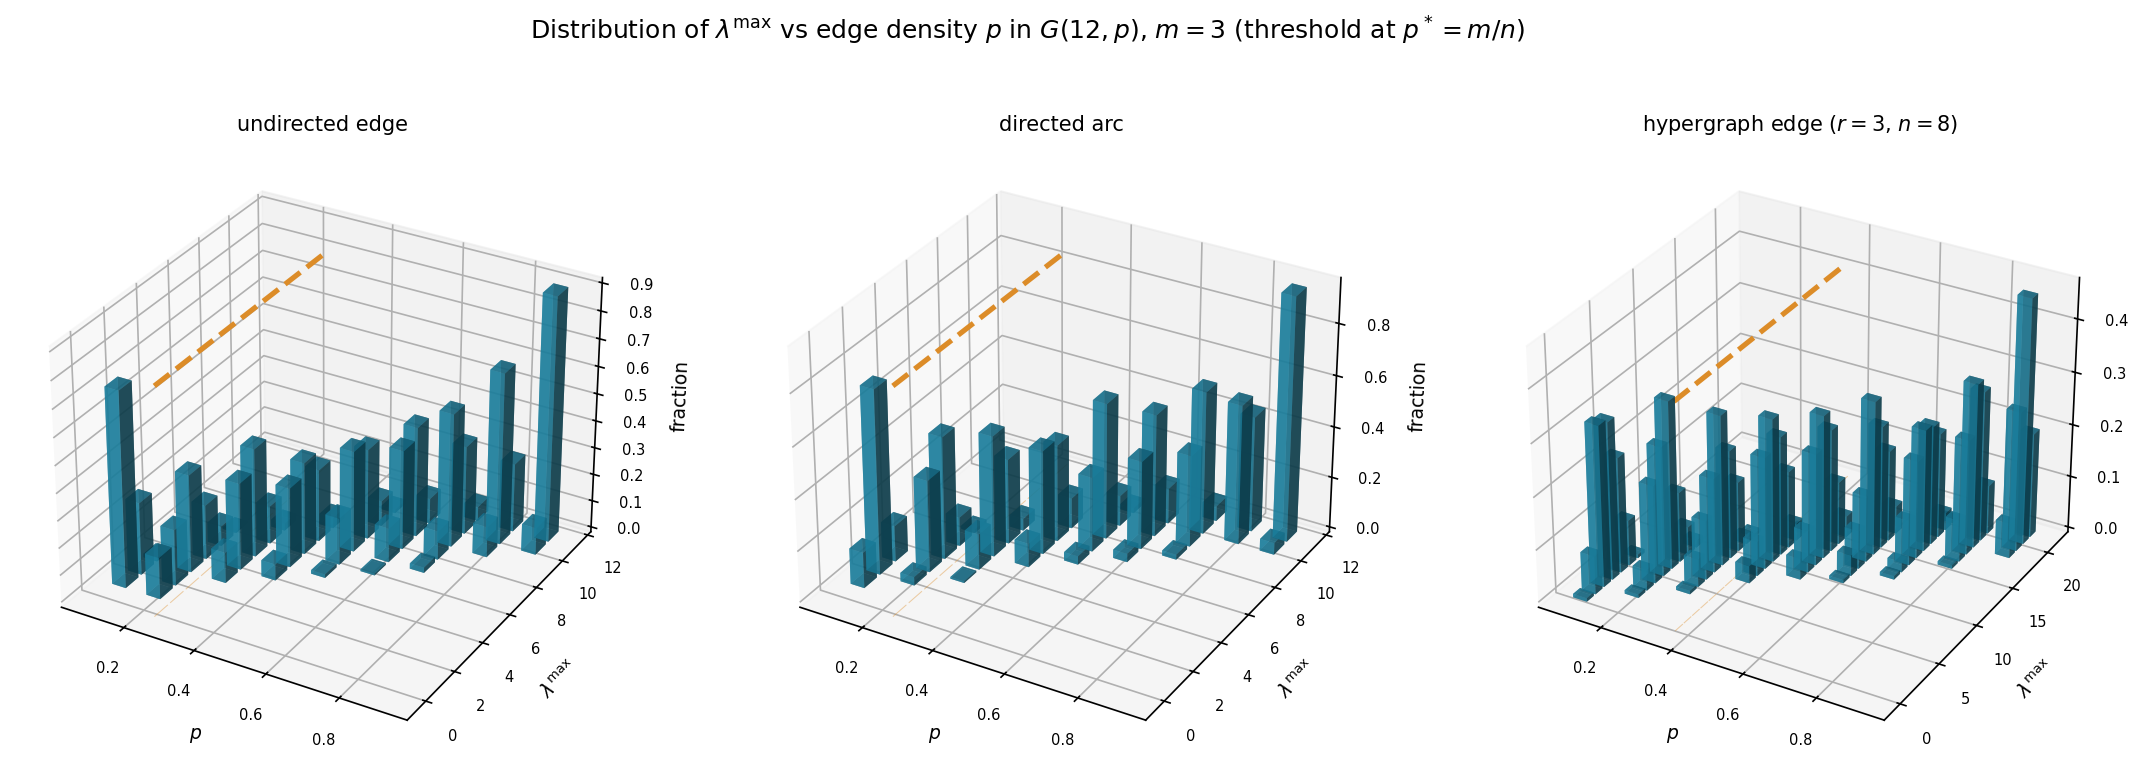
\includegraphics[width=0.86\textwidth]{figures/threshold_3d.png}
    \caption{The appearance threshold of \Cref{fig:threshold} as a three-dimensional bar chart, for three representative variants (simple undirected edge, simple directed arc, three-uniform hypergraph edge) at $n = 12$, $m = 3$. Each panel plots the fraction of $G(n, p)$ samples (height) reaching each binding connectivity $\lambda^{\max}$ (depth) as the density $p$ varies (width), so the mass migrates from low to high connectivity as $p$ crosses the proved threshold $p^* = m/n$. File \code{threshold\_3d.png}.}
    \label{fig:threshold-3d}
\end{figure}
